\section{Act 3: Visualizing and analyzing ET data with GMEMs and GAMMs}

In all previous steps, wrangling can be thought of as a condensing process, where the primary object is to remove, clean, and transform the data into a structure that is usable. However, once the data is put into tidy form, then the data must be transformed for specific  visualizations and analyses. In this section, we think of \inlineR{all\_data\_cleaned} and \inlineR{all\_data\_tidy} as launching points to gain understanding of our data. 

For data visualization, it is often necessary to put the data into a form that is quite different than the cleaned data, either through aggregation,by filtering, or splitting into multiple data frames. In L: 395, we begin such an example of aggregation for visualization. Here, our goal is to create a visualization to compare looks to targets in different conditions (e.g., looks to targets for \inlineR{verb\_type} restricting vs. \inlineR{verb\_type} non-restricting sentences). In L: 397 we group by participant, condition, and time to prepare for aggregating mean looks to targets, competitors and distractors in L: 397-400. L:400 is created as a raw count for the calculation of empirical logits in L:402-403.

\lstinputlisting[style=mystyle, firstnumber=last]{scripts/chunk-All Data: Preparing for Visualization.R}

For \inlineR{ggplot()} visualizations, see \inlineR{AOW\_r\_work\_flow.rmd}. We observed nearly identical time course of predictive processing, see figure \ref{fig:smooth}, in which restricted sentences resulted in earlier looks to the target object than nonrestrictive sentences. Further, this effect is even partially reduced in accented speech in a similar manner to \textcite{Porretta_et_al_2020}. 

\begin{figure}[h]
    \centering
    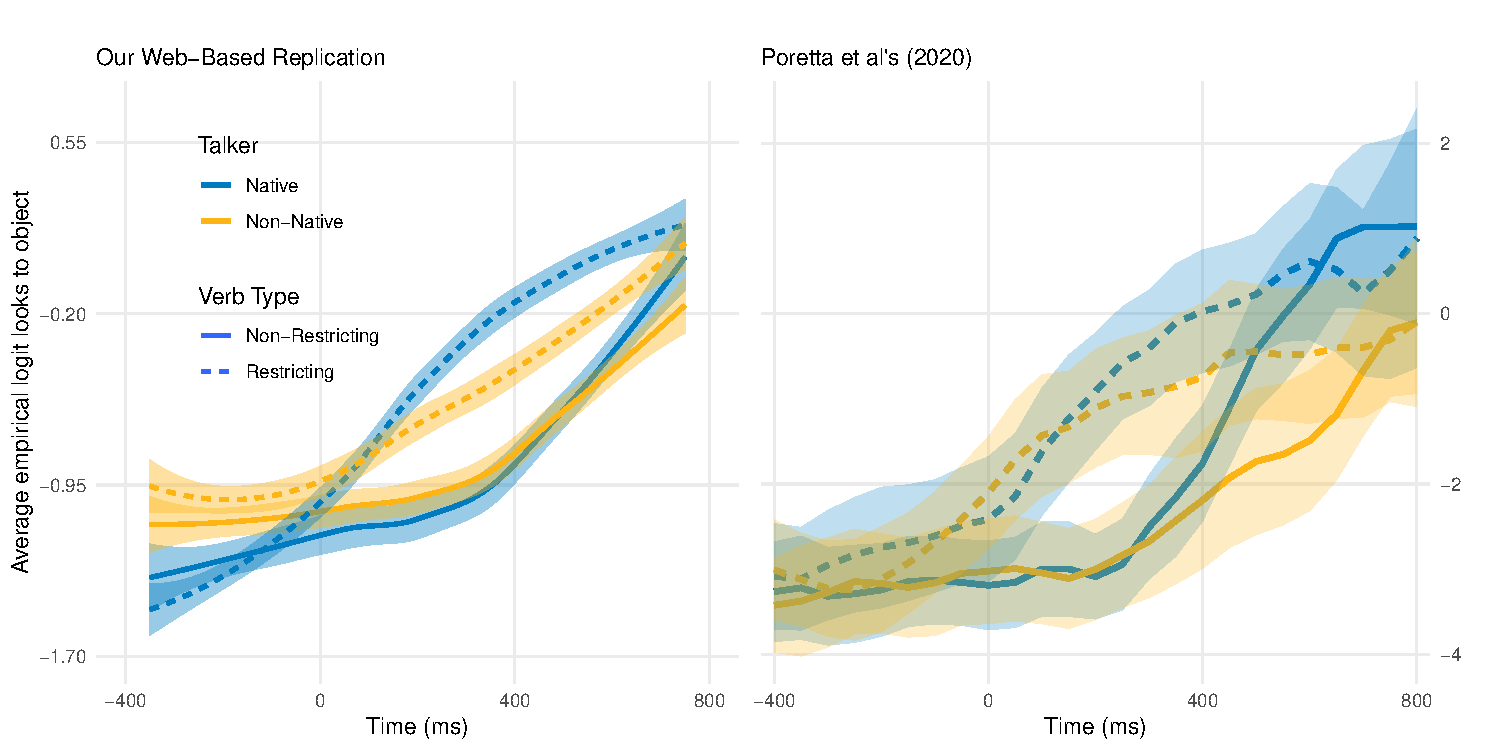
\includegraphics[width=\textwidth]{figures/smooth_comparison_plot.pdf}
    \caption{Left: our Data. right \parencite{Porretta_et_al_2020}}
    \label{fig:smooth}
\end{figure}

 Here, we are creating two data frames from \inlineR{all\_data\_tidy}: \inlineR{mem\_data} in L: 405 and then \inlineR{gamm\_data} in L: 411. In general in data wrangling, keeping as much data as possible is essential to creating a usable data frame. However, in model wrangling, it is often best to remove variables that you will not be using. This is because some models can have issues being interpreted through unprocessed data types. For \inlineR{mem\_data},we start by selecting all necessary columns for the model: \inlineR{Participant.Private.ID}, \inlineR{verb\_type},\inlineR{talker},item \inlineR{subject\_img\_file},\inlineR{target},log frequency of object item\inlineR{log\_SUBTLWF\_Obj}, and  \inlineR{ time\_elapsed\_rounded}. \inlineR{Participant.Private.ID} is turned into a factor in L:48. Finally, \inlineR{tidy\_quest\_data} is joined to \inlineR{mem\_data}. In addition to the \inlineR{mem\_data}, we create \inlineR{gamm\_data} by simply cloning \inlineR{mem\_data} in L:411 and by adding a single variable needed in the GAMM models

\lstinputlisting[style=mystyle, firstnumber=last]{scripts/chunk-All Data: Preparing for Models.R}

GAMMS and GLMERS both have there own advantages and disadvantages \parencite{Ito_Knoeferle_2022}. GLMERS means generalized linear Mixed effect Models. The models are logistic regression models that estimate both fixed and random effects. GLMERS are simple to use, flexible and provide highly interpretable results. Further, they offer powerful insight into data that can be assumed to be linear. In contrast, GAMMs (generalized linear mixed effects models) are able to model both linear and non-linear data. more here.

Both GLMER and GAMMS require specific coding of the data for the model to predict in the expected manner. However, each of these models start with coding the data correctly and building maximal models and working down to simpler models for model comparison. \parencite{max model}.

\subsection{GLMERs}

For GLMERs coding 

\lstinputlisting[style=mystyle, firstnumber=last]{scripts/chunk-GLMER: Leveling the Data.R}


GLMER Models were built using the lme4 package \parencite{Bates2014-eq}. The models included three fixed effects: \inlineR{verb\_type} (Restrictive or Non-Restrictive), \inlineR{talker}(Native, Non-Native) and their interaction. \inlineR{verb\_type}(Restrictive) and \inlineR{talker}-Native were set as reference levels. All variables were coded with
effects coding L: 413-417. Random intercepts for \inlineR{subject\_img\_file},\inlineR{time\_normalized}, and
\inlineR{Participant.Private.ID} were included, as were random slopes for \inlineR{talker} and \inlineR{verb\_type}, but correlations were removed after model comparison showed preference for simpler model with lower AIC.





\lstinputlisting[style=mystyle, firstnumber=last]{scripts/chunk-GLMER: Leveling the Data.R}


%Mixed-effect logistic regression was carried out in R [6], formula: glmer(target ~ talker accent * verb type + (1| item)+(verb type||Participant), family= binomial)). Like [1]’s model, our model yielded an effect of verb type for the restrictive condition (β = 0.08, SE = .04, t = 2.28, p = .029) indicating that prediction occurs irrespective of accent. Additionally, our model found neither an effect of talker accent nor a two-way interaction, thus mirroring the results of [1].

\begin{figure}[h]
    \centering
    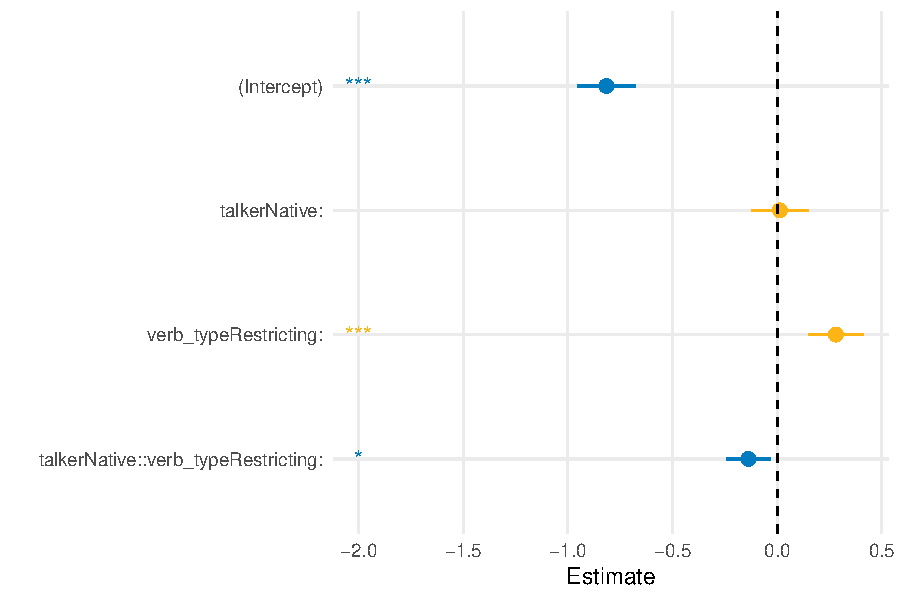
\includegraphics[width=\textwidth]{figures/GLMER_base_model.pdf}
    \caption{place holder for real model outputs later}
    \label{fig:model_outputs}
\end{figure}

\begin{figure}[h]
    \centering
    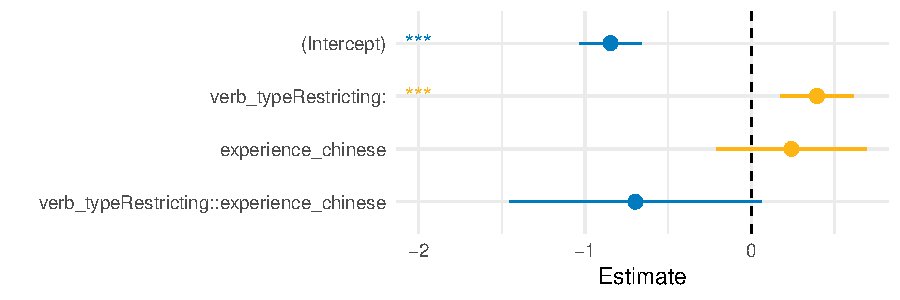
\includegraphics[width=\textwidth]{figures/GLMER_accent_model.pdf}
    \caption{place holder for real model outputs later}
    \label{fig:model_outputs}
\end{figure}

\subsection{Growth Curve Analysis}

Another possible model to use is Growth curve analysis. Prolly not cause space but it seems so logical here. glmer:linear-> GCA:manual polynomials (relax linearity)-> GAMM:automated polynomials (forget about linearity)


\subsection{Generalized Additive Modeling}

\lstinputlisting[style=mystyle, firstnumber=last]{scripts/chunk-GAMM: Leveling the Data.R}


GAMMS are becoming increasingly popular as they allow the research to model complex time course information without the need for assumptions of linearity.

include comparitive visual of 
\begin{figure}[h]
    \centering
    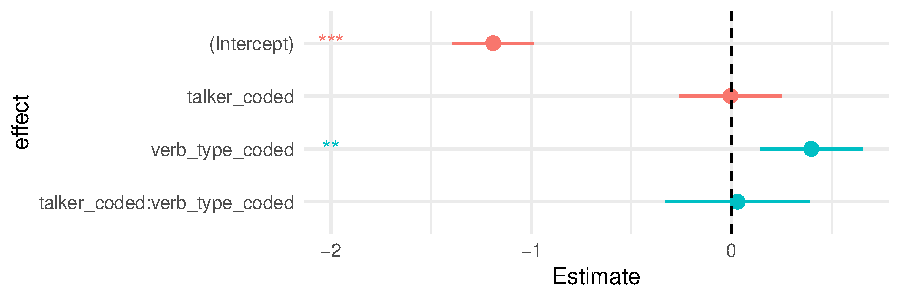
\includegraphics[width=\textwidth]{figures/model_gamm_effects.pdf}
    \caption{place holder for real model outputs later}
    \label{fig:model_outputs}
\end{figure}